
% this file is called up by thesis.tex
% content in this file will be fed into the main document

%: ----------------------- introduction file header -----------------------
\begin{savequote}[50mm]
Now this is not the end. It is not even the beginning of the end. But it is, perhaps, the end of the beginning. 
\qauthor{Winston Churchill}
\end{savequote}


\chapter{Conclusions}
\label{cha:Conclusions}

\ifpdf
    \graphicspath{{6_conclusion/figures/PDF/}}
\fi

This chapter reviews the most significant results of this thesis, remarking the 
specific contributions and identifying several further research areas. First, 
an introduction discussing the contributions detailed during this dissertation 
is presented. These contributions are described in Section~\ref{sec:contributions}. 
Besides, several publications that support the different elements presented in 
this dissertation are enumerated in Section~\ref{sec:publications}.


\section{Discussion}
\label{sec:discussion}

This thesis arises from a series of problems identified in 2010, when Imhotep
was developed as a response to the observed demand of adaptive user interfaces 
solutions for people with disabilities. Dealing with the available technology
and analysed approaches a solution in which developers were given an \ac{api}
for developing adaptive interfaces was designed. Based on preprocessor primitives,
developers were able to include pieces of source code in which user interface
configuration were completed with a user and a device profile. Those profiles
were given by the potential users through another application.

Imhotep was highly accepted by the scientific community. Several publications
were produced (as shown in Section~\ref{sec:publications}) and an award was 
given based on the AssistedCity developed use case.

However, in spite of the success of Imhotep, technology improvements regarding
mobile devices bring new challenges and possibilities. Thus, from the weaknesses
of Imhotep new solutions arose. These challenges were which conceived AdaptUI.

First, a further analysis of the literature and state of the art in user 
interface adaptation solutions was needed. The lack of mobile based user 
interface adaptive solutions was identified. Besides, the current ongoing 
software and hardware mobile devices improvements enhanced the design of a 
mobile platform.

After taking the decision of using a mobile centred platform, the challenge of
what and how to model arose. Based on our previous experience and on the reviewed
literature a semantic model based on three entities was conceived. This model
mainly combines user's interaction characteristics, a current context situation
description, and different device's characteristics. As one of the identified
problems in the analysed user adaptation platforms in the literature is their
lack of independence from the considered domain, a semantic based design determined.
This allows an easy method to represent the knowledge of the domain, extend it,
share it, and adapt it to any desired sub-domain by just combining different 
ontologies with the provided AdaptUIOnt.

The combination of the two previous mentioned decisions brought a significant
problem: the lack of available mobile based semantic reasoning engines. Therefore,
as a technical contribution AdaptUI provides a mobile reasoning engine based on
Pellet and compatible with Android. It is called \textit{Pellet4Android}, it is
open source, and it provides support for \ac{owl} 2 and \ac{swrl} rules in Android.

Once the semantic models and the mobile semantic infrastructure for reasoning
were operative, the required architecture was design, as is shown in Figure~\ref{fig:architecture_discussion}.

\begin{figure}[H]
\centering
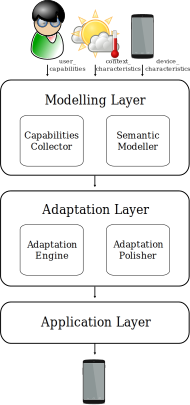
\includegraphics[width=0.30\textwidth]{architecture.pdf}
\caption{AdaptUI's three-layered global architecture.}
\label{fig:architecture_discussion}
\end{figure}

Besides, in order to make AdaptUI accessible for developers, two main \acp{api}
are provided. These \acp{api} aim to allow developers not only to adapt the
user interfaces of their application, but also to adapt the whole AdaptUI platform
to the domain they work with.

% In this thesis several contributions have been provided: First, in 
% Chapter~\ref{cha:ontology_model}, the AdaptUIOnt ontology has been presented. 
% AdaptUIOnt is an ontology that models user interaction capabilities, context 
% current situation and device characteristics with a design that allows a dynamic 
% update of the represented knowledge. Second, \textit{Pellet4android} has been
% introduced in Chapter~\ref{cha:architecture}. \textit{Pellet4android} is a 
% semantic reasoning engine based on Pellet but compatible with Android devices.
% Finally, AdaptUI, a whole dynamic user interface adaptation platform, which 
% allows developers to design adaptive user interfaces for their applications, has 
% been described.

% As AdaptUIOnt has been first highlighted, in the following lines we summarize 
% several conclusions and benefits of the cited designed ontology:
% In the following lines we summarize several conclusions and benefits of AdaptUIOnt:
% 
% \begin{itemize}
%   \item AdaptUIOnt arises from the identified weaknesses of the models and solutions
%   reviewed in Chapter~\ref{cha:state_of_the_art}. Centred on the user needs, it
%   models several characteristics that define users, context and devices, 
%   regarding the current needs for the interaction with the current user 
%   interface, and allowing their semantic representation. 
% 
%   \item AdaptUIOnt allows the modelling of non physiological interaction 
%   capabilities of the user. As mentioned in Chapter~\ref{cha:state_of_the_art}, 
%   several solutions aiming the adaptation of user interfaces (or services) 
%   take into account user physiological capabilities. However, these solutions 
%   assume that these capabilities are properly provided by the user or by 
%   external services. But the truth is that, analysing these solutions, no 
%   experts are consulted or included in the researches. Thus, to us these 
%   solutions, although they are interesting, do not cover the reality of the 
%   users and their daily limitations when dealing with interaction activities. 
%   Hence, the AdaptUIOnt ontology has been designed taking into account this 
%   issue. By avoiding the inclusion of physiological knowledge about user's 
%   capabilities we allow users to directly manipulate their applications without 
%   considering specific expertise or medical background. Besides, developers do 
%   not have to consult any expert in the area, as the translation of the user 
%   interactions are represented in the ontology as preferences and needs, not as 
%   capabilities.
% 
%   \item It allows the addition of external ontologies to complete the knowledge 
%   of the main entities. One of the benefits of semantic representation is the
%   ability to join external ontologies which can enrich the knowledge base. Thus,
%   developers are allowed to design their models or use those ontologies they
%   prefer to better fit AdaptUI in their domains. For example, \textit{Context}
%   has not been designed from scratch. Several extra ontologies, fully supported
%   and used by the community, have been used to build the corresponding knowledge
%   about the context. 
% \end{itemize}
% 
% As the AdaptUI platform is based on semantics and reasoning, a mobile reasoning 
% engine is required. The ported \textit{Pellet4Android} reasoning engine provides
% several benefits, all inherited from Pellet for Java. Although, as is remarked
% in Chapter~\ref{cha:evaluation}, more tests are needed to assure a similar
% performance in mobile devices. Nevertheless, this port provides:
% 
% \begin{itemize}
%   \item Representation and reasoning about information using \ac{owl} in Android
%   based mobile devices.
%   
%   \item Support for \ac{owl} 2 for Android devices.
%   
% %   \item 
% \end{itemize}
% 
% Finally, regarding the whole AdaptUI platform:
% 
% \begin{itemize}
%   \item It allows users to configure the best suitable adaptation regarding their 
%   capabilities, temporary disabilities, context current characteristics and
%   their devices' dynamic and static set of characteristics. Through a simple
%   application they are able to configure the best user interface combination
%   of components for each case. These configurations are stored in the ontology,
%   indexed by the context disabilities extracted from the reasoning process. 
%   Thus, each time AdaptUI detects a known context situation and reasons over 
%   it. If the same disabilities are sensed, they corresponding user interface 
%   is adapted.
%   
%   \item It also allows developers to forget about the aspect of their applications, regarding
%   inclusive design and adaptation, as the platform automatically manages it. 
%   Besides, they are allowed to modify the knowledge through the provided 
%   \acp{api}. Classes, properties, individuals and rules are fully modifiable, 
%   which gives total liberty to developers to adapt the whole platform to their 
%   needs.
%   
%   \item It provides a fully 100\% mobile adaptation platform. It does not require external
%   processing aid, nor even Internet connectivity. Due to the 
%   \textit{Pellet4Android} reasoning engine every reasoning and semantics
%   management process runs in the mobile. This fact avoids possible failures due
%   to connectivity or network losses.
% \end{itemize}

Although AdaptUI has several benefits and it contributes with the mentioned 
completed goals, the presented platform has also several constraints:

\begin{itemize}
  \item Depending on the hardware of the used devices might lead into 
  performance penalization if such devices have not the necessary computing
  capabilities. Although the results presented in 
  Chapter~\ref{cha:evaluation} brought promising references regarding device's 
  processing capabilities, the less powered device is a Samsung Galaxy SIII Mini.
  
  \item Although we have demonstrated that several temporary context 
  disabilities and limitations are considerably reduced, people with 
  disabilities might still suffer several interaction problems. Thus, further 
  efforts are needed to improve and finalise the whole system. This issue is 
  described in Section~\ref{sec:future_work}.
  
  \item Another limitation is that AdaptUI mostly considers disabilities based
  on visual and hearing constraints. Although others have been studied (as motor
  disabilities), the experiments are difficult to carry out. This is also 
  detailed in Section~\ref{sec:future_work}, as we aim to cover more limitations 
  and experiment with such contexts.
\end{itemize}


\section{Contributions}
\label{sec:contributions}

A summary of the different contributions described in this thesis is presented 
in this section: 

\begin{enumerate}[label=\alph*)]
  \item In Chapter~\ref{cha:state_of_the_art} an in-depth analysis of the state 
  of the art is presented:
  \begin{itemize}
    \item Evaluating several approaches to modelling and reasoning over user,
    context and device.
    \item Analysing several adaptive and adaptable solutions in the field of
    user interfaces.
    \item Studying these solutions architectures and possibilities considering
    nowadays technology.
    \item This covers the objective 1 detailed in Section~\ref{sec:hypothesis}.
  \end{itemize}
  
  \item In Chapter~\ref{cha:ontology_model} an ontology for modelling users, 
  context, devices and the corresponding user interface adaptations is presented.
  \begin{itemize}
    \item Allowing the inclusion of adaptation rules to manage the adaptation 
    process.
    \item Avoiding the explicit user physiological capabilities modelling.
    \item Providing a dynamic design to allow the platform to dynamically update
    the corresponding entity.
    \item The results of this chapter accomplishes the goal specified in the
    objectives 2 and 3 in Section~\ref{sec:hypothesis}.
  \end{itemize}

  \item Chapter~\ref{cha:architecture} presents an Android compatible mobile 
  reasoning engine based on Pellet, and the corresponding architecture
  for enabling the dynamic user interface adaptation supporting semantics.
  \begin{itemize}
    \item Providing a full Pellet port available for Android devices.
    \item Allowing the use of semantics and \acp{swrl} compatible reasoning.
    \item Describing the different modules which power the whole system.
    \item Including the decisions consequences and their conclusions.
    \item This covers all the objectives mentioned in Section~\ref{sec:hypothesis},
    as it provides the necessary infrastructure to build the whole adaptation
    platform.
  \end{itemize}

%   \item Chapter~\ref{cha:architecture} introduces the corresponding architecture
%   for enabling the dynamic user interface adaptation supporting semantics.
%   \begin{itemize}
%     \item Describing the different modules which power the whole system.
%     \item Including the decisions consequences and their conclusions.
%     \item This covers all the objectives mentioned in Section~\ref{sec:hypothesis},
%     as it provides the necessary infrastructure to build the whole adaptation
%     platform.
%   \end{itemize}

  \item Finally the previous contributions where combined to offer an 
  implementation of a dynamic user interface adaptation system that provides a 
  more practical and complete vision of the user interaction capabilities.
  
\end{enumerate}


\section{Publications and Awards}
\label{sec:publications}

The contributions of this thesis have been presented to the scientific community 
in a series of international forums, such as: journals and conferences.

\subsection{International \acs{jcr} Journals}

% The current versions of the AdaptUI mobile user interface adaptation 
% system were published in the following journals:

\begin{itemize}
  \item Castillejo, E., Almeida, A., {López-de-Ipiña}, D., 2014. Ontology Based 
  Model for Supporting Dynamic and Adaptive User Interfaces. International 
  Journal of Human-Computer Interaction 30, 771–786. 
  doi:10.1080/10447318.2014.927287.


  \item Eduardo Castillejo, Aitor Almeida, Diego {López-de-Ipiña} and Liming Chen. 
  Modeling Users, Context and Devices for Ambient Assisted Living 
  Environments. Sensors, MDPI. vol. 14, no. 3, pp. 5354-5391, \acs{doi}: 
  10.3390/s140305354, \acs{issn} 1424-8220, \acs{jcr} Impact Factor (2012): 1.953, 
  January 2014.
  
  \item Eduardo Castillejo, Aitor Almeida, and Diego {López-de-Ipiña}. Modelling 
  users, context and devices for adaptive user interface systems. International 
  Journal of Pervasive Computing and Communications 10, no. 1 (January 2014): 
  5-5
\end{itemize}
  
As mentioned before, this dissertation arises from the weaknesses and future work
identified in previous research works. 

\begin{itemize}
  \item Aitor Almeida, Pablo Orduña, Eduardo Castillejo, Diego {López-de-Ipiña} 
  and Marcos Sacristan. A method for automatic generation of fuzzy membership 
  functions for mobile device’s characteristics based on Google Trends. 
  Computers in Human Behaviour (Journal). Volume 29, Issue 2. Pages 510–517. 
  Impact Factor (2011): 2.293 \acs{doi}: 10.1016/j.chb.2012.06.005. March 2013.
  
  \item Aitor Almeida, Pablo Orduña, Eduardo Castillejo, Diego {López-de-Ipiña}, 
  Marcos Sacristán. Imhotep: an approach to user and device conscious mobile 
  applications. Personal and Ubiquitous Computing (Journal). Volume 15, Issue 
  4, pp 419–429. Springer. Impact Factor (2009): 1.554. \acs{issn}: 1617-4909. 
  \acs{doi}: 10.1007/s00779-010-0359-8. January 2011.
\end{itemize}


\subsection{International Conferences}

As this thesis started as a result of previous research work related to user 
interface adaptation, the following publications are included:

\begin{itemize}
  \item Aztiria, A., Castillejo, E., Almeida, A., {López-de-Ipiña}, D., 2014. 
  Adapting user interfaces based on user preferences and habits, in: 
  Proceedings of the 10th International Conference on Intelligent Environments 
  (IE14). Presented at the 10th international conference on Intelligent 
  Environments (IE14), Shangai, China.


  \item Aitor Almeida, Pablo Orduña, Eduardo Castillejo, Diego {López-de-Ipiña}, 
  and Marcos Sacristán. An approach to automatic generation of fuzzy 
  membership functions using popularity metrics. In Information Systems, 
  E-learning, and Knowledge Management Research, pp. 528-533. Springer Berlin 
  Heidelberg, 2013.
  
  \item Aitor Almeida, Pablo Orduña, Eduardo Castillejo, Diego {López-de-Ipiña}, 
  Marcos Sacristán. Adaptative applications for heterogeneous intelligent 
  environments. ICOST 2011: 9th International Conference on Smart Homes and 
  Health Telematics. Montréal, Canada, June 2011. LNCS6719, Toward Useful 
  Services for Elderly and People with Disabilities, Springer, \ac{isbn}: 
  978-3-642-21534-6, pp. 1-8.
  
  \item Aitor Almeida, Pablo Orduña, Eduardo Castillejo, Diego {López-de-Ipiña}, 
  Marcos Sacristán. A user-centric approach to adaptable mobile interfaces 
  Actas del II International Workshop of Ambient Assisted Living (IWAAL 2010), 
  p.p. 153-160 Valencia, Spain, September 7-10, 2010 (\ac{isbn}: 978-84-92812-67-7).
\end{itemize}


\subsection{Awards}
\label{sec:awards}

AssitedCity, the use case developed using the Imhotep framework for adaptive
user interfaces was awarded in March 7, 2012 with the Via Inteligente 
award\footnote{http://www.viainteligente.com/premios2012.html}. This prize was 
possible thank to the collaboration with Dr. Aitor Almeida and Dr. Pablo Orduña, 
and thank to the supervision of Dr. Diego López-de-Ipiña. 
% The previous work carried out with Dr. Aitor Almeida, Dr. Pablo Orduña and  
% with the Imhotep framework was awarded in March 7, 2012 with the Via Inteligente 
% award.


\section{Future Work}
\label{sec:future_work}

Although all the accomplishments covered by AdaptUI, there are still several 
areas and features in which more efforts are required to improve the presented 
results. Consequently, in this section we present several ideas about future 
research actions and, in some cases, an explanation of the the steps that have 
been already taken are given.

\begin{enumerate}[label=\alph*)]
  \item Dynamic self-generation adaptive rules. Although AdaptUI provides three 
  different sets of rules, these rules are static, and they always depend on 
  the corresponding developer to be designed. This means that rules have to 
  be added in a previous stage, when users are still not present. In the near 
  future we aim to provide to AdaptUI an extra module capable of generate and 
  adapt in running time different rules considering several context change 
  triggers. Thus, from a default set of rules, these rules would be personalized 
  through the user experience.
  
  \item A further \textit{Pellet4Android} evaluation and tests are needed. The
  provided Pellet based mobile reasoning engine seeks functionality. Therefore,
  although it provides promising results running in Android devices, deeper 
  stress and  more complex processing experiments are planned. A deeper
  comparison of both versions of Pellet should produce more concluding results.
  
  \item AdaptUI basically covers disabilities related to visual and hearing
  sensory limitations. A further study and analysis of these and more 
  disabilities, based on the \ac{icf} document [], would include more users and 
  better adaptations of the user interfaces.
\end{enumerate}

\section{Final Remarks}
\label{sec:final_remarks}

This dissertation is the result of years of research including several areas
within the \acl{aui} field. With it, I have tried to contribute
with significant improvements considering the current state of the art. Besides,
I deem that these contributions will further help a more widespread adoption of 
adaptive user interfaces design for users with disabilities. I also hope that 
this thesis will inspire and contribute to the scientific community, as others 
have undoubtedly inspired me. 
% ----------------------------------------------------------------------


